\section{NC $\pi^0$ Rate Validation }
\label{sec:deficit}

NC $1\pi^0$ events contribute as a dominant background to NC single-photon production measurements carried out or planned by MicroBooNE such as searches for NC $\Delta$ radiative decay \cite{MicroBooNE:2021zai}, NC coherent single-photon production, or more rare $e^{+}e^{-}$ pair production motivated in BSM theories. In addition to using these selected events as a calibration sample for understanding and validating shower reconstruction performance, they are also used to validate the observed overall rate of this process as currently modeled with \textsc{genie}. Assuming \textsc{genie} provides a sufficient description of the observed data, this sample can and has been used to provide an \textit{in situ} constraint on NC $1\pi^0$ mis-identified backgrounds, \textit{e.g.}~as in \cite{MicroBooNE:2021zai}. Alternatively, these measurements can be used to increase our understanding of our current NC $\pi^0$ modelling and potentially motivate \textsc{genie} tuning.

As shown in Fig.~\ref{fig:ncpi0_costheta}, both the $2\gamma1p$ and the $2\gamma0p$ selections see an overall deficit in data relative to the MC prediction. This is more pronounced in the $2\gamma1p$ selection where the ratio of the number of selected data events to the number of selected simulated events is 0.79. As it is also known that the \textsc{genie} branching fraction of coherent NC $1\pi^{0}$ production on argon is significantly lower than expectation extrapolated from MiniBooNE's $\pi^{0}$ measurement on mineral oil~\cite{MiniBooNE:2008mmr}, the possibility of a correction to \textsc{genie} predictions on both non-coherent and coherent NC $1\pi^0$ production is explicitly examined. The MC predictions are fitted to data allowing both coherent and non-coherent NC $1\pi^{0}$ rates to vary. Both normalization-only and normalization plus shape variations to the coherent and non-coherent rates are explored; all yield similar conclusions. This section describes the normalization plus shape variation fit in detail.  

The normalization plus shape variation fit is performed as a function of reconstructed $\pi^0$ momentum for both 2$\gamma1p$ and $2\gamma0p$ selections, using [0, 0.075, 0.15, 0.225, 0.3, 0.375, 0.45, 0.525, 0.6, 0.675, and 0.9] GeV/c bin limits. In the fit, MC predicted coherent NC $1\pi^0$ events are scaled by a normalization factor $N_{coh}$, and MC predicted non-coherent NC $1\pi^0$ events are scaled on an event-by-event basis depending on their corresponding true $\pi^0$ momentum according to $(a+b|\vec{p}^{~true}_{\pi^{0}}|)$, where the true $\pi^0$ momentum is given in [GeV/c]. This linear scaling as a function of $\pi^0$ momentum was chosen because it was the simplest implementation that was consistent with the observed data-to-MC deficit, as observed in Fig.~\ref{fig:ncpi0_mom_2g1p}.

At each set of fitting parameters ($N_{coh}$, $a$, $b$), a $\chi^2$ is evaluated between the scaled prediction for this parameter set and the observed data using the Combined-Neyman-Pearson $\chi^2$ \cite{Ji:2019yca}. The $\chi^2$ calculation makes use of a covariance matrix including statistical and systematic uncertainties and correlations corresponding to the scaled prediction. Flux, cross section, detector and \textsc{geant4} systematic uncertainties are included in the fit including bin-to-bin systematic correlations. As the goal of the fit is to extract the normalization and scaling parameters of the coherent and non-coherent NC $1\pi^{0}$ rates, the cross-section normalization uncertainties of coherent and non-coherent NC $1\pi^{0}$ are not included. Note that the cross-section normalization uncertainties of coherent and non-coherent NC $1\pi^{0}$ are only removed for the purposes of this fit and not for the cross section extraction described in the following section. 

The data-extracted best-fit parameters correspond to $a=0.98$ and $b=-1.0$~[c/GeV] for the scaling parameters of the non-coherent NC $1\pi^0$ events, and $N_{coh}=2.6$ for the NC coherent $\pi^0$ normalization factor with no enhancement, $N_{coh}=1$, being allowed within the $1\sigma$ error bands. This best-fit gives a $\chi^2$ per degree of freedom ($dof$) of 8.46/17. The $\chi^2/dof$ at the \textsc{genie} central value (CV) prediction is 13.74/20 yielding a $\Delta\chi^2$ between the \textsc{genie} CV and the best-fit point of 5.28 for 3 $dof$. Although the goodness-of-fit $\chi^2/dof$ values for both scenarios are acceptable due to the generally large uncertainties, the momentum-dependent shift is preferred over the \textsc{genie} CV at the 1.43$\sigma$ level. The 1D marginalized $\Delta\chi^2$ distributions in Fig.~\ref{fig:marginalized_chi} also confirm that the \textsc{genie} CV prediction agrees with data within uncertainty. The data and MC comparisons of the reconstructed $\pi^0$ momentum distributions scaled to the best-fit parameters are provided in Fig.~\ref{fig:momentum_BF} and, compared to those corresponding to the \textsc{genie} CV, show better agreement with data after the fit.

\begin{figure}[h!]
  \begin{subfigure}{0.49\textwidth}
  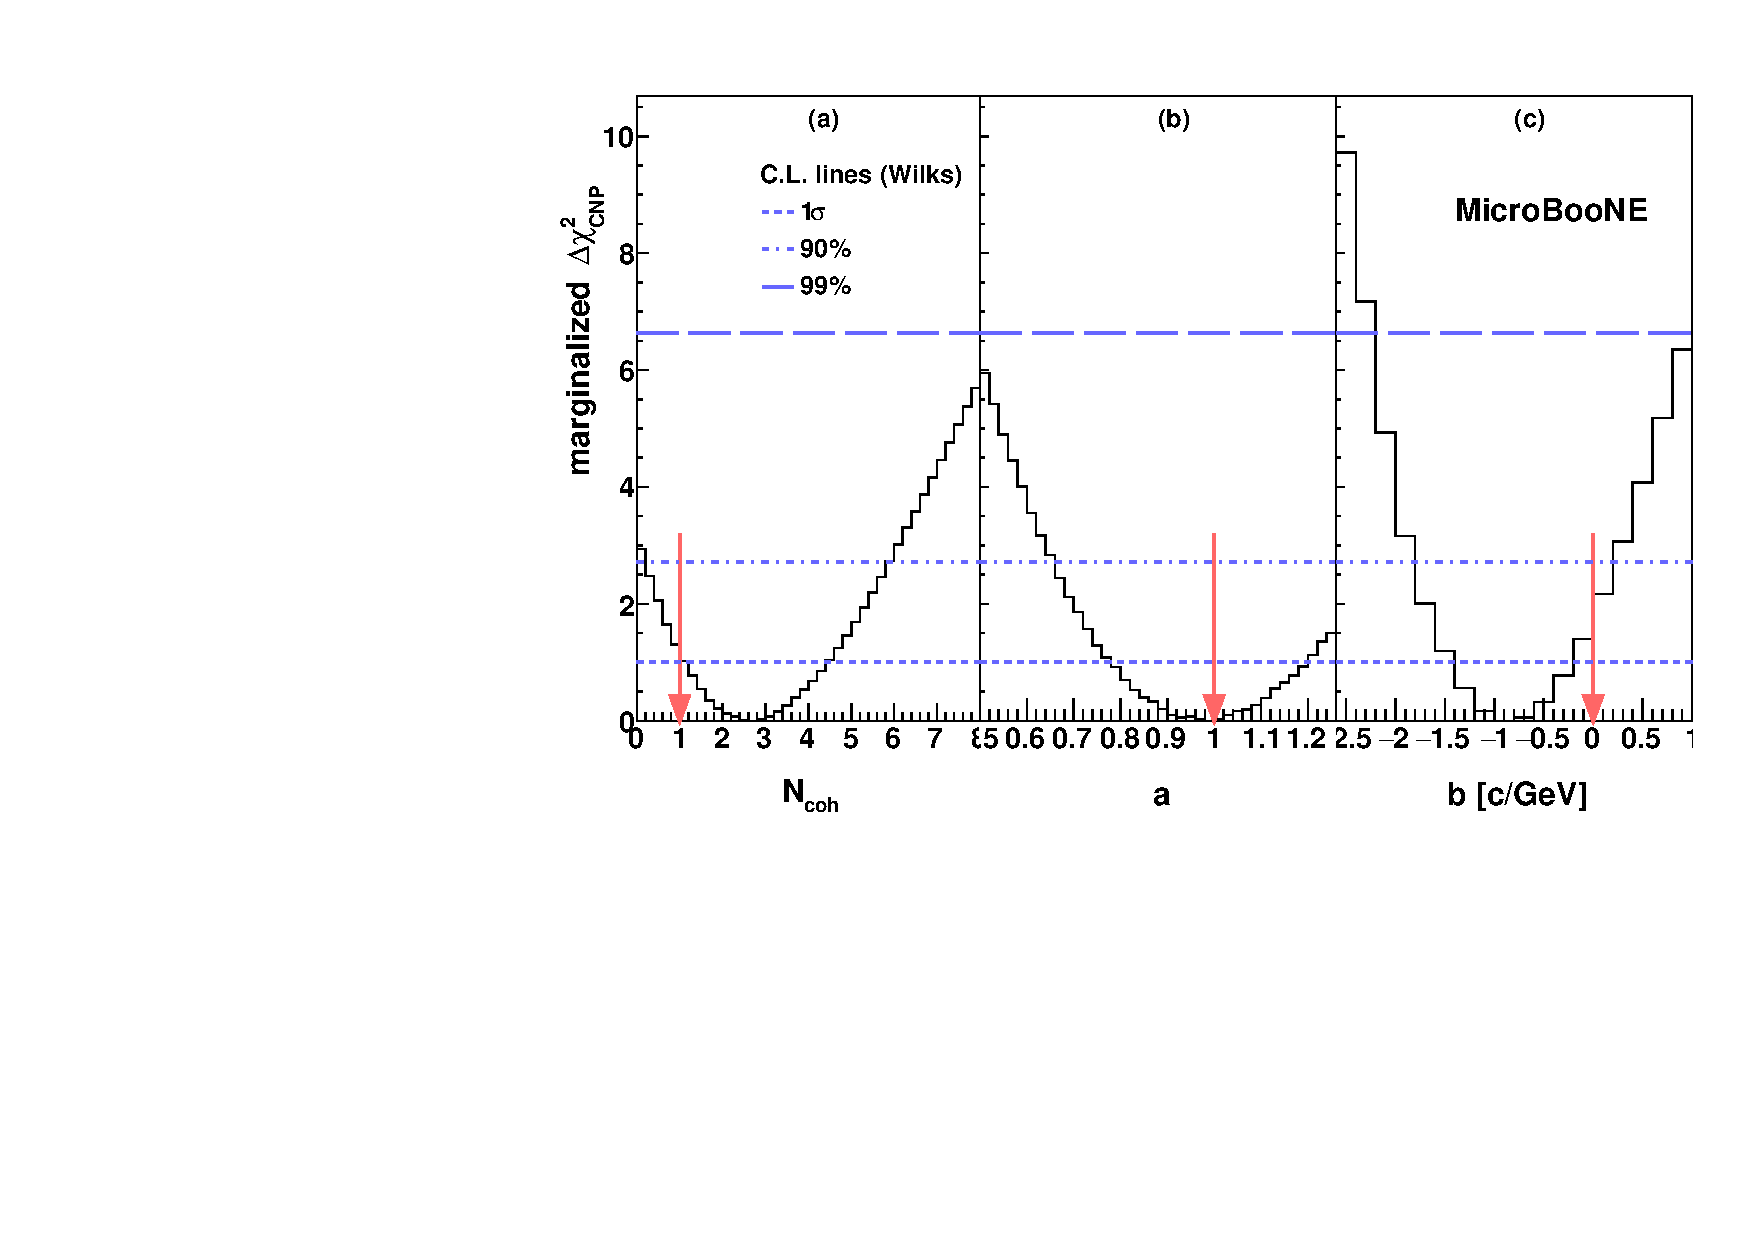
\includegraphics[width = \textwidth]{fig10_Marginalized_chi_distribution_uboone.pdf}
  \end{subfigure}
\caption{The distribution of marginalized $\Delta\chi^2$, as a function of flat normalization factor for (a) coherent NC 1$\pi^0$ momentum-independent scaling factor, (b) non-coherent NC 1$\pi^0$ momentum-independent scaling factor, and (c) coefficient of momentum-dependent scaling factor for NC non-coherent 1$\pi^0$, marginalized over the other two parameters. The red arrows indicate parameter values expected for the \textsc{genie} central value prediction. The 1$\sigma$, 90\% and 99\% C.L.~lines are based on the assumption that the distribution follows a $\chi^2$ distribution with 1 degree of freedom.
}
\label{fig:marginalized_chi}
\end{figure}


\begin{figure}[h!]
  \begin{subfigure}{0.49\textwidth}
   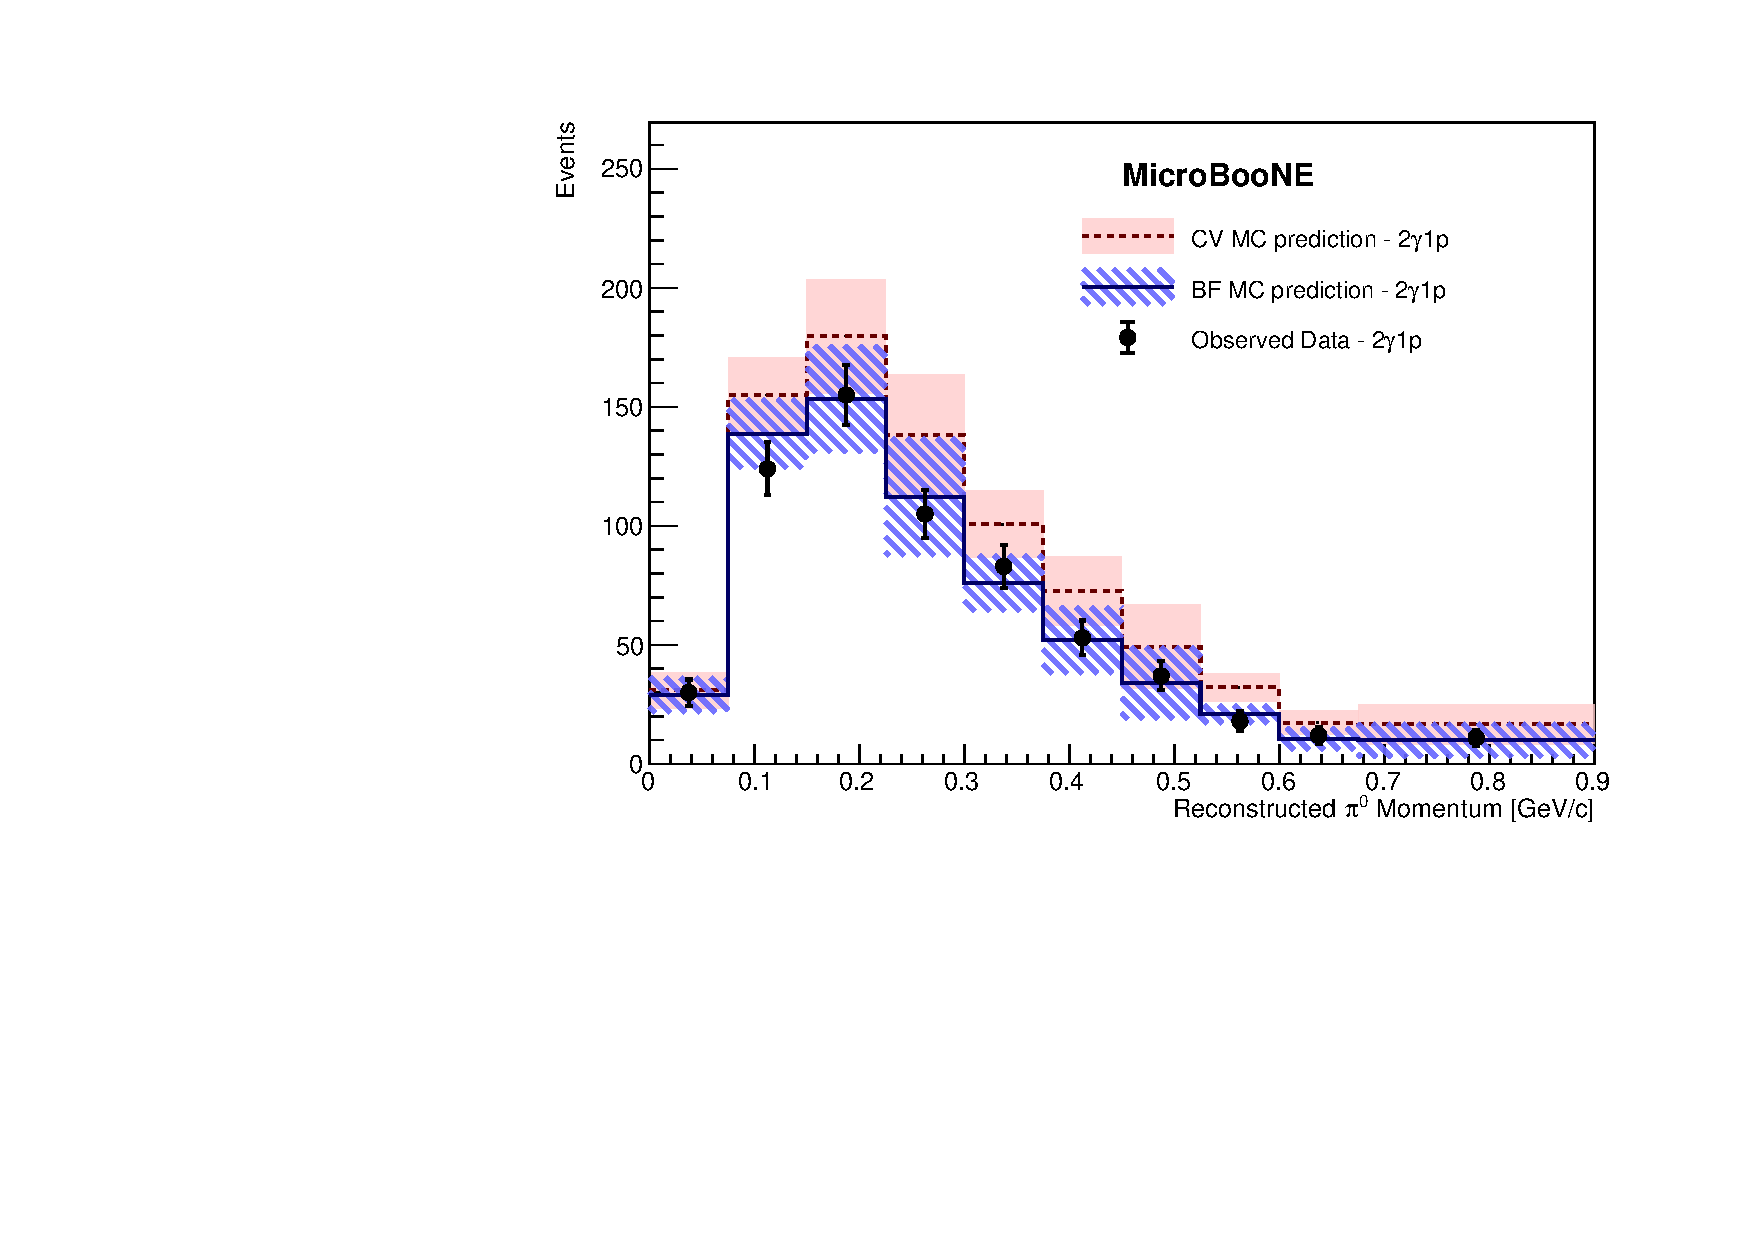
\includegraphics[width = \textwidth]{fig11a_Data_MC_comparison_2g1p_uboone.pdf}
  \caption{$2\gamma1p$}
  \end{subfigure}%
  
  \begin{subfigure}{0.49\textwidth}
   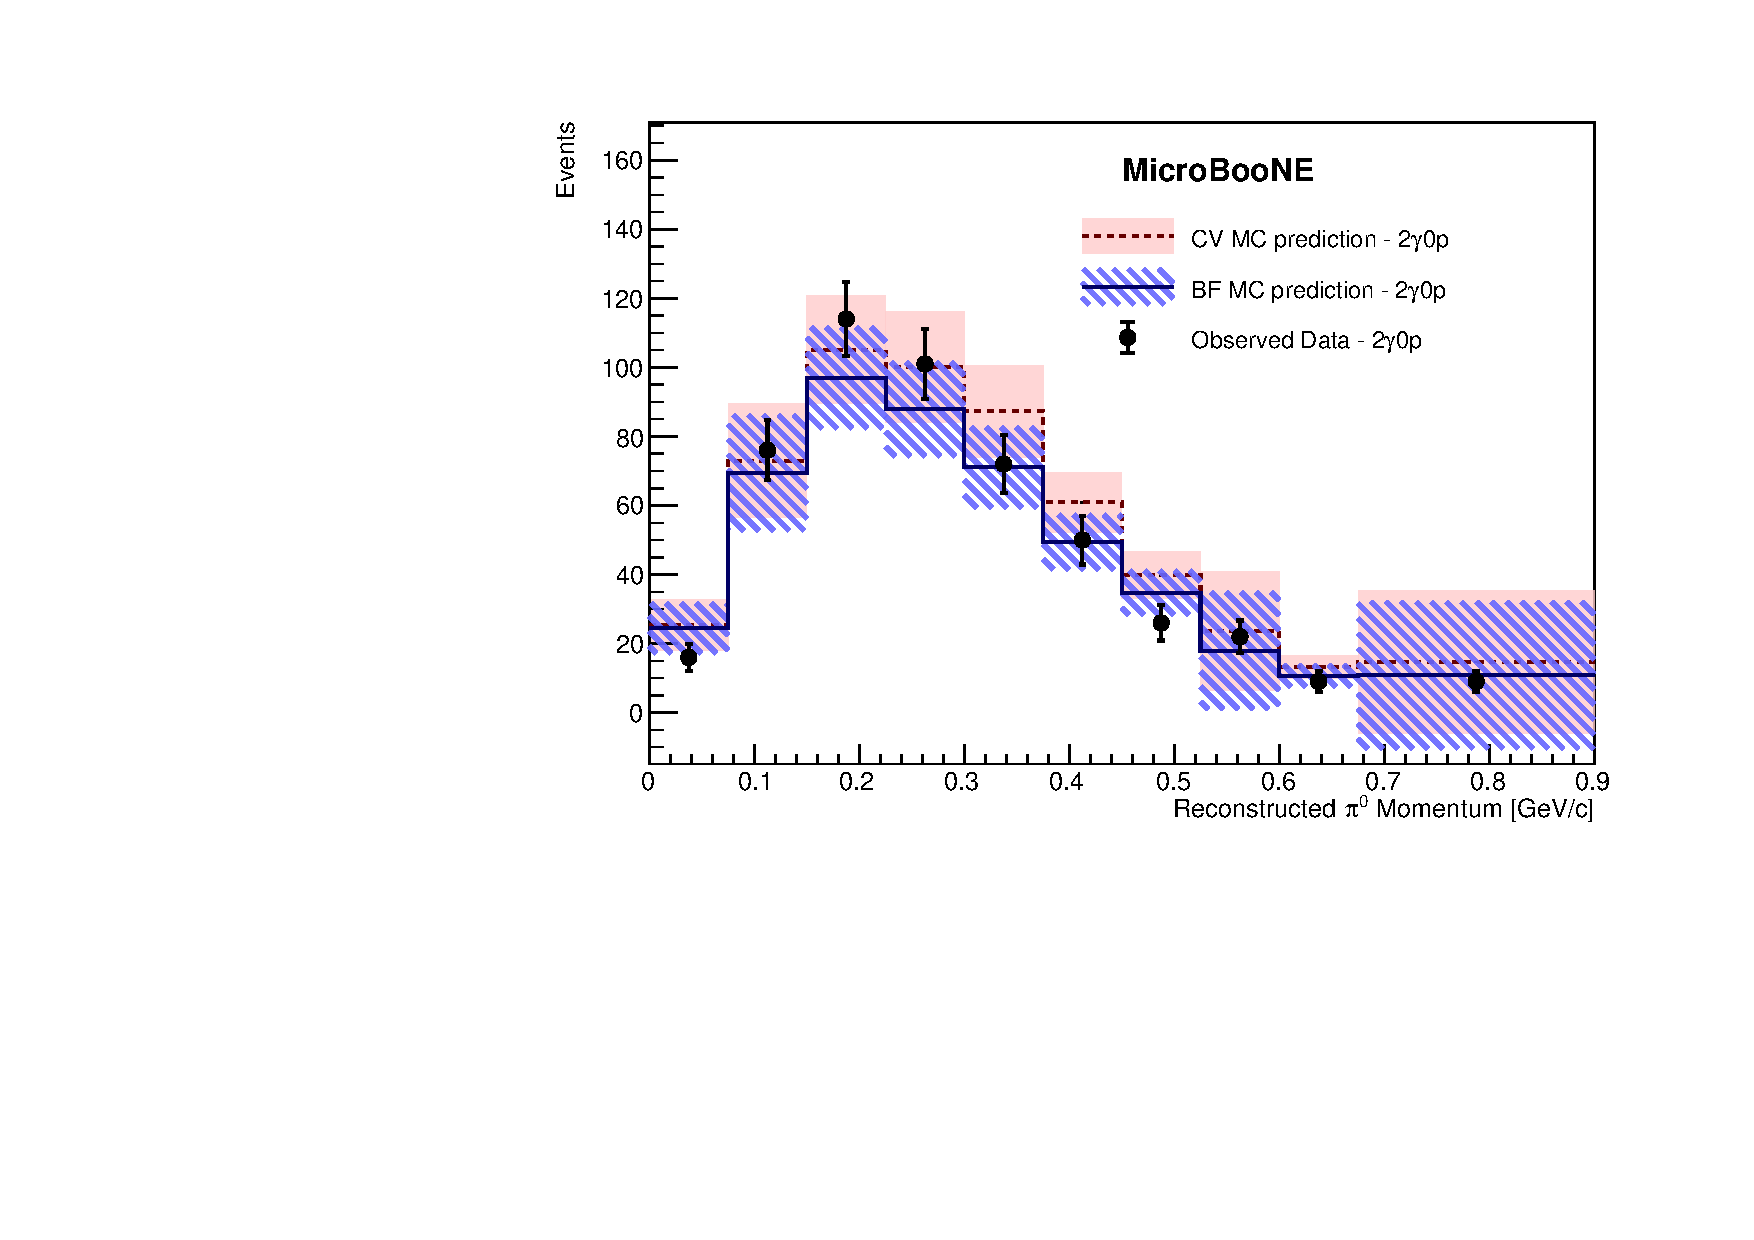
\includegraphics[width = \textwidth]{fig11b_Data_MC_comparison_2g0p_uboone.pdf}
  \caption{$2\gamma0p$}
  \end{subfigure}
  \caption{The data-MC comparison for (a) $2\gamma1p$ and  (b) $2\gamma0p$ selections, as a function of reconstructed $\pi^0$ momentum. Monte Carlo predictions at the central value and at the best-fit point ($\text{N}_{coh} = 2.6$, $a=0.98$, $b=-1.0$~[c/GeV]) are both shown, with prediction and corresponding systematic error evaluated at the \textsc{genie} central value in salmon, and at the best-fit in blue. Note that the systematic uncertainties on the plot include MC intrinsic statistical error and all the systematic errors (flux, cross-section and detector), with the exception of cross section normalization uncertainties on coherent and non-coherent NC 1$\pi^0$.}
  \label{fig:momentum_BF}
\end{figure}


While the data suggest that \textsc{genie} may over-estimate NC $1\pi^0$ production, the results demonstrate that the \textsc{genie} prediction of NC $1\pi^{0}$s is accurate within uncertainty. This validates the approach of using the measured NC $1\pi^{0}$ event rate as a powerful \textit{in situ} constraint of \textsc{genie}-predicted NC $1\pi^0$ backgrounds as in \cite{MicroBooNE:2021zai}.  We stress that while this result motivates a momentum dependent shift in how we model our NC $\pi^0$ events, we do not apply this change to our modeling, relying instead on the fact that the assigned uncertainty covers the observed discrepancy. Future work will investigate further the possibility of tuning \textsc{genie} with results such as these to obtain better model predictions. On the other hand, it is natural to extract a data-driven NC 1$\pi^{0}$ cross-section on argon using these selections, and compare to a number of neutrino event generators, including \textsc{genie}. This is described below. 


 


